\begin{frame}[fragile]
  \frametitle{Solution Attempt 1 - cell-level}
  The charge expected on the \textbf{wires} ($\vec{w}$) can be calculated
  given (the unknown) charge in the \textbf{cells} ($\vec{c}$):

  \[\vec{w} = \mathbf{G_{wc}}\vec{c}\]

  $\mathbf{G_{wc}}$ is the \textbf{wire-cell adjacency matrix}, purely
  geometrical and perfectly known, function of detector design.
  
  \begin{columns}
    \begin{column}{0.45\textwidth}
      \vspace{-5mm}

      \flushright 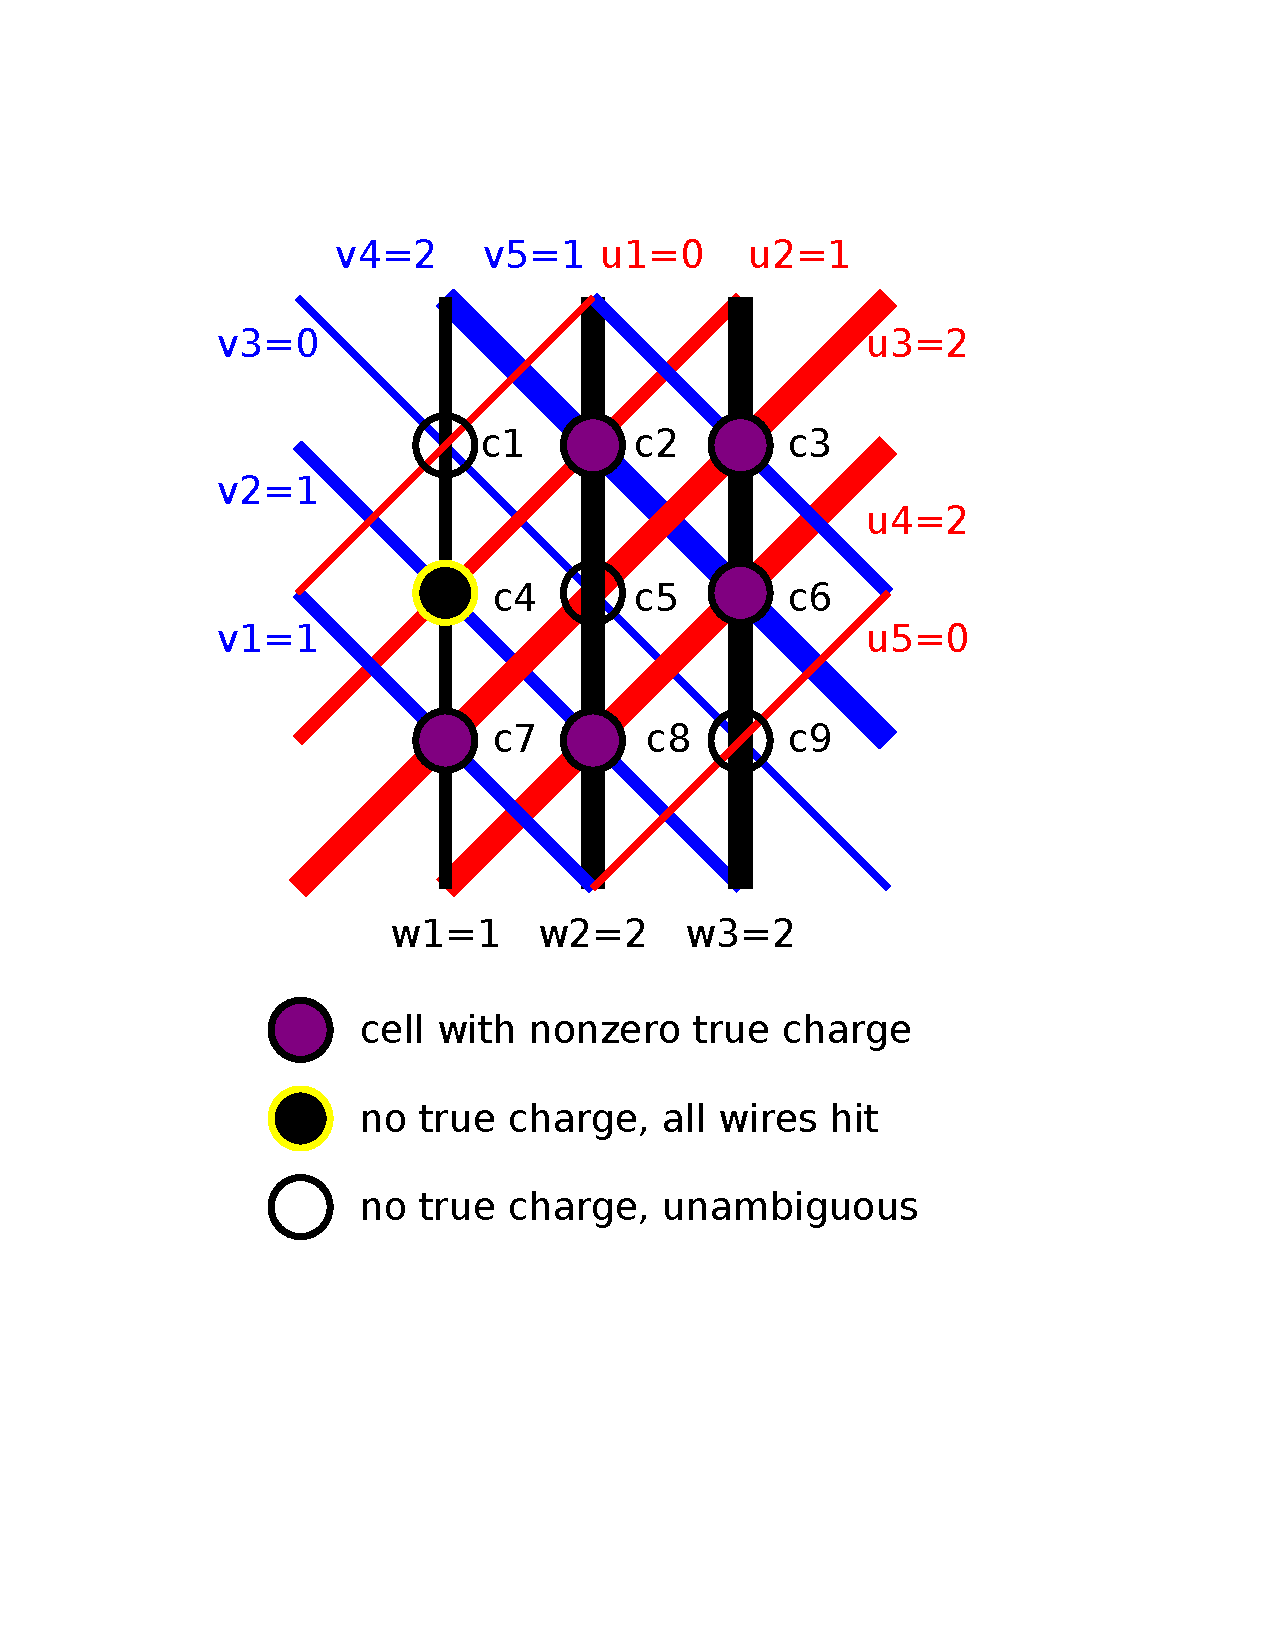
\includegraphics[width=0.8\textwidth,trim=1cm 11cm 2cm 2cm,clip]{example-hit-cells.pdf}

    \end{column}
    \begin{column}{0.10\textwidth}
      $\Leftrightarrow$
    \end{column}
    \begin{column}{0.45\textwidth}

  \resizebox{0.7\textwidth}{!}{
    $\left(
      \begin{array}[h]{c}
        0.0\\
        1.0\\
        2.0\\
        2.0\\
        0.0\\

        1.0\\
        1.0\\
        0.0\\
        2.0\\
        1.0\\

        1.0\\
        2.0\\
        2.0\\
      \end{array}
    \right)
    = \left(
      \begin{array}[h]{ccccccccc}
        1&0&0&0&0&0&0&0&0\\
        0&1&0&1&0&0&0&0&0\\
        0&0&1&0&1&0&1&0&0\\
        0&0&0&0&0&1&0&1&0\\
        0&0&0&0&0&0&0&0&1\\

        0&0&0&0&0&0&1&0&0\\
        0&0&0&1&0&0&0&1&0\\
        1&0&0&0&1&0&1&0&0\\
        0&1&0&0&0&1&0&0&0\\
        0&0&1&0&0&0&0&0&0\\
        
        1&0&0&1&0&0&1&0&0\\
        0&1&0&0&1&0&0&1&0\\
        0&0&1&0&0&1&0&0&1\\
      \end{array}
    \right)
    \left(
      \begin{array}[h]{c}
        0.0\\
        1.0\\
        1.0\\
        0.0\\
        0.0\\
        1.0\\
        1.0\\
        1.0\\
        0.0\\
      \end{array}
    \right)$}
      
    \end{column}
  \end{columns}


  Wish to solve inverse: $\vec{c} = \mathbf{G}^{-1}_{\mathbf{wc}}\vec{w}$.
  However, $N_{cells} \approx N_{wires}^2$ \\
  $\Rightarrow$ as $N_{cells}$ grows, more unknowns ($\vec{c}$) than knowns ($\vec{w}$)!
\end{frame}


\begin{frame}[fragile]
  Wire Cell uses a \textbf{tomographic} approach to produce a
  model-free \textbf{3D image} of activity in the LAr.

  \vfill
  Example:

  \begin{columns}

    \begin{column}{0.5\textwidth}
      \begin{center}
        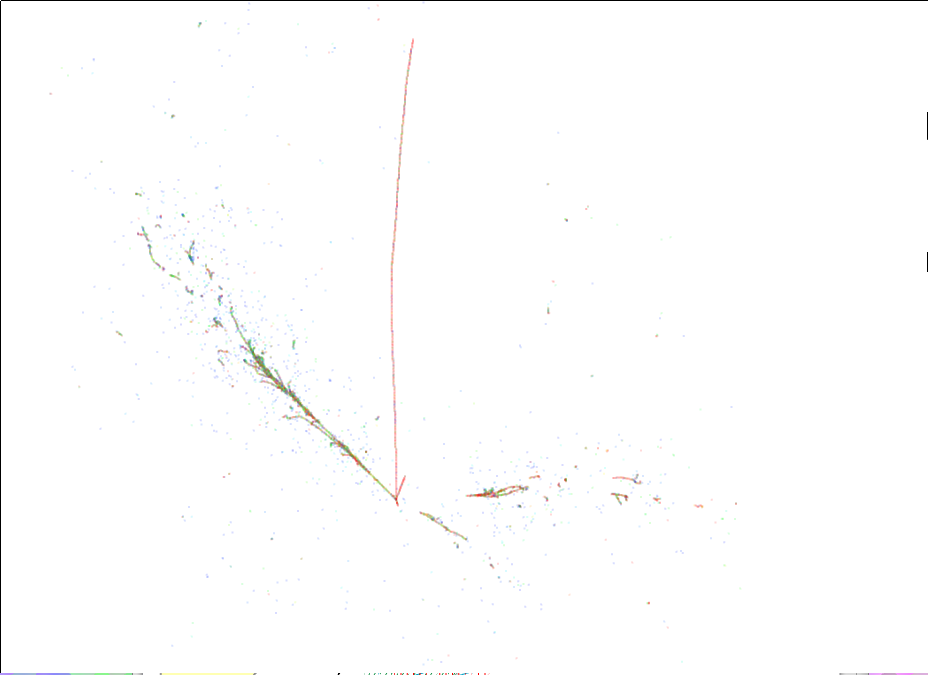
\includegraphics[trim=1cm 2cm 1cm 2mm, clip, height=45mm]{bee-true.png}\\
        True energy deposits.
      \end{center}
    \end{column}

    \begin{column}{0.5\textwidth}
      \begin{center}
        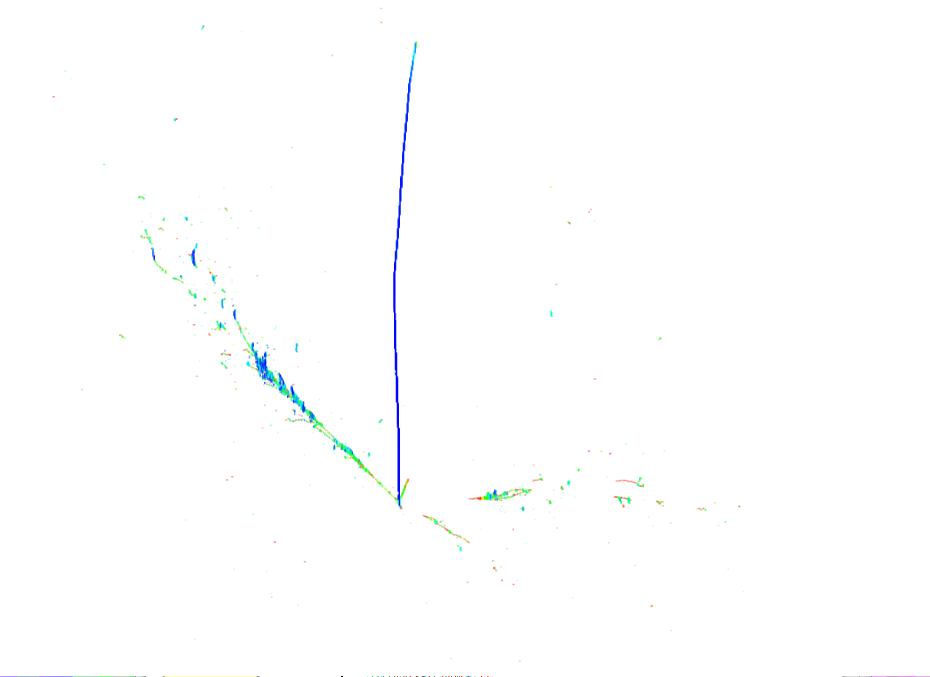
\includegraphics[trim=1cm 2cm 1cm 2mm, clip, height=45mm]{bee-reco.png}\\
        Wire Cell imaging.
      \end{center}
      
    \end{column}
  \end{columns}

  \vfill

\end{frame}



\begin{frame}[fragile]
  \frametitle{Source Repositories and Build}

  \begin{itemize}
  \item Code in GitHub \href{https://github.com/WireCell/}{WireCell} organization.
  \item Code aggregation with \texttt{git submodule}.
  \item A simple, customized \href{https://waf.io/}{waf}-based build.\footnote{\texttt{wcb} = \texttt{waf} + extra Waf tools for Boost, ROOT, Eigen and Wire Cell packaging}
  

  \end{itemize}

  \begin{lstlisting}{langauge=shell}
$ git clone git@github.com:WireCell/wire-cell.git
$ cd wire-cell/
$ git submodule init
$ git submodule update
$ ./wcb --prefix=/path/to/install configure build install
  \end{lstlisting}
%$

  Builds, tests and installs:
  \begin{itemize}
  \item toolkit shared libraries + header files,
  \item no main applications yet but many, unit+integration tests
  \end{itemize}
  Also: \href{http://www.phy.bnl.gov/wire-cell/doxy/html/}{Doxygen code reference} and \href{http://wirecell.github.io/wire-cell-docs/}{MkDocs user documentation}.


\end{frame}

\begin{frame}[fragile]
  \frametitle{Wire Cell Interfaces}

  The \href{https://github.com/WireCell/wire-cell-iface}{\texttt{wire-cell-iface}} package:

  \begin{itemize}
  \item API composed of abstract base classes covering:
    \begin{itemize}
    \item \textbf{Data model} (wires, cells, frames, slices, tracks, ...)
    \item \textbf{Active components} (blob maker, matrix solver, clustering, ...)
    \end{itemize}
  \item Pervasive use of C++ \verb|shared_ptr<>| for (mostly) \textbf{worry-free memory management}.
  \item Dynamic instance lookup via \texttt{NamedFactory} pattern
    allows for a \textbf{plugin architecture}.
  \item Initial support for \textbf{user configuration} system based on Boost
    property trees.
  \item Initial support exists for an \textbf{abstract execution model}.
    \begin{itemize}\scriptsize
    \item[$\rightarrow$] more on this coming up.
    \end{itemize}
  \end{itemize}
\end{frame}

\begin{frame}

  \frametitle{Wire Cell Simulation}

  \begin{columns}
    \begin{column}{0.75\textwidth}
      \begin{itemize}\footnotesize
      \item Provided by the \href{https://github.com/WireCell/wire-cell-gen}{\texttt{wire-cell-gen}} package.
      \item Simple implementation of the 4 ``D''s of LArTPC:\\
        \textbf{deposit, drift, diffuse, digitize}.
      \item Granular, use as little or as much as needed.
        \begin{itemize}\scriptsize
        \item[$\rightarrow$] Parts can be replaced by \textbf{external
          simulation}, \\or bypassed entirely with \textbf{real DAQ data}.
        \item[$\rightarrow$] \textbf{External integration} via file I/O or API calls.
        \end{itemize}
      \item Provides reference implementation to guide integrator/developers of external frameworks.
      \item Useful for quickly generating data to feed unit tests.
      \end{itemize}
    \end{column}
    \begin{column}{0.25\textwidth}
      \vspace{-10mm}
      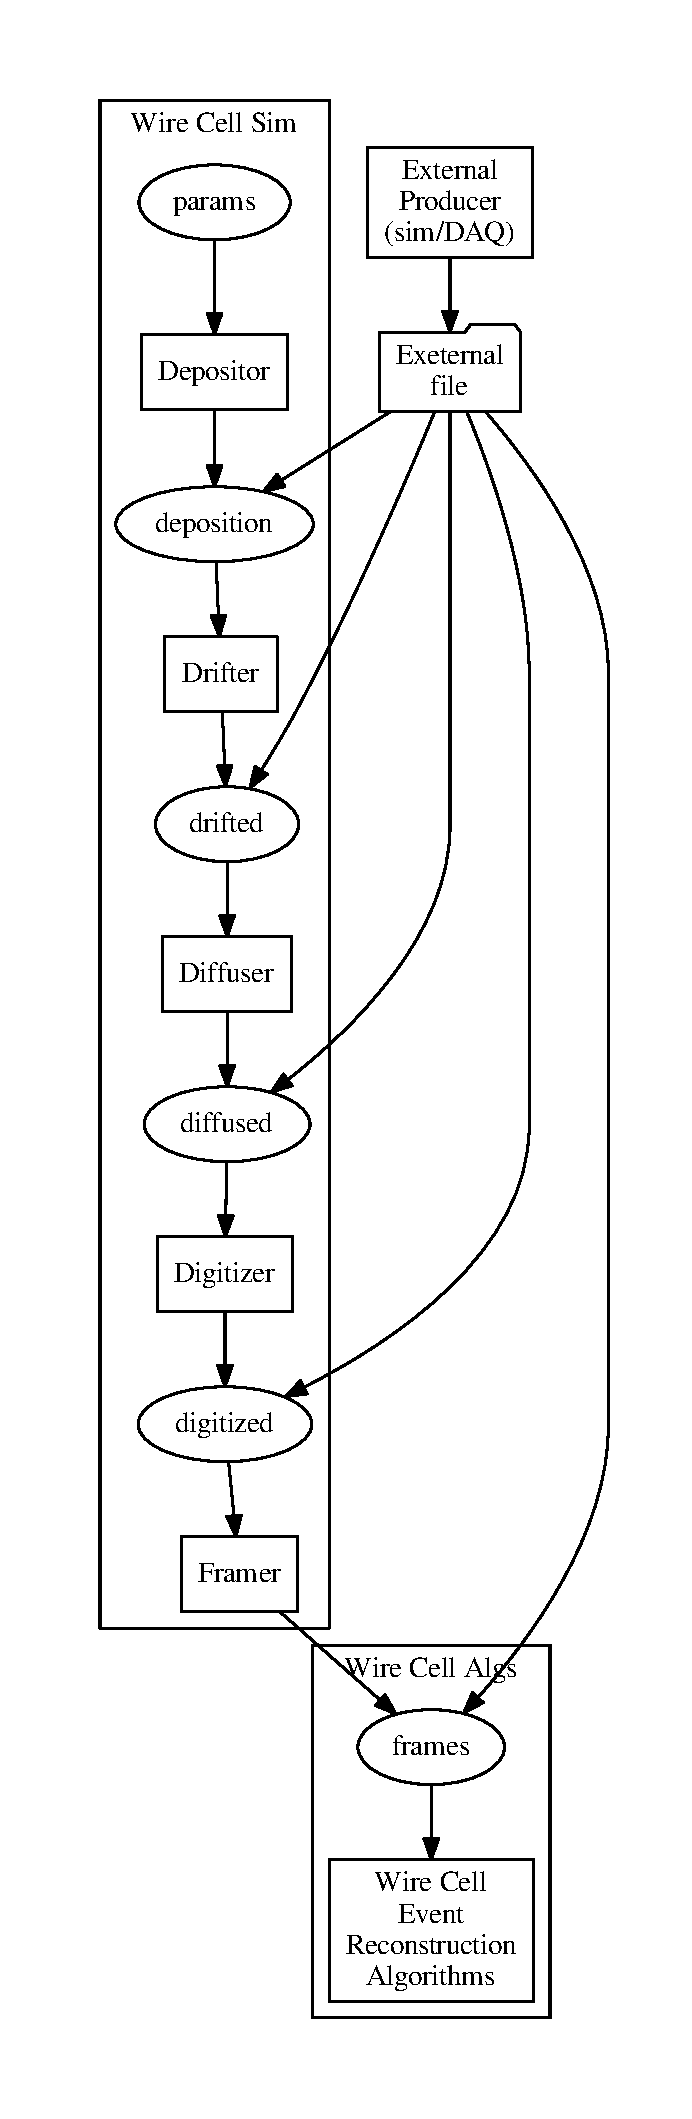
\includegraphics[width=\textwidth]{sim-flow.pdf}
    \end{column}
  \end{columns}
\end{frame}

\begin{frame}
  \frametitle{Abstract execution model}

  \scriptsize Want ability to change execution model while leaving ``real'' algorithm code untouched!

\footnotesize
  
  \begin{columns}
    \begin{column}{0.65\textwidth}
      Each graph vertex made from \textbf{three layers}.\\

      \vspace{2mm}

      From outside to in:
      \begin{enumerate}
      \item Execution model layer implementing the data flow control
        \begin{itemize}\scriptsize
        \item sync'ed load-and-flush, async, multi-processing, message-passing, ...
        \item some implementations identified
        \end{itemize}
      \item Adapter wraps actual algorithm and presents uniform
        interface to execution model layer.
      \item Algorithm implementation and interface left unrestricted
        except ``no shared globals'' (thread safety).
      \end{enumerate}
    \end{column}
    \begin{column}{0.35\textwidth}
      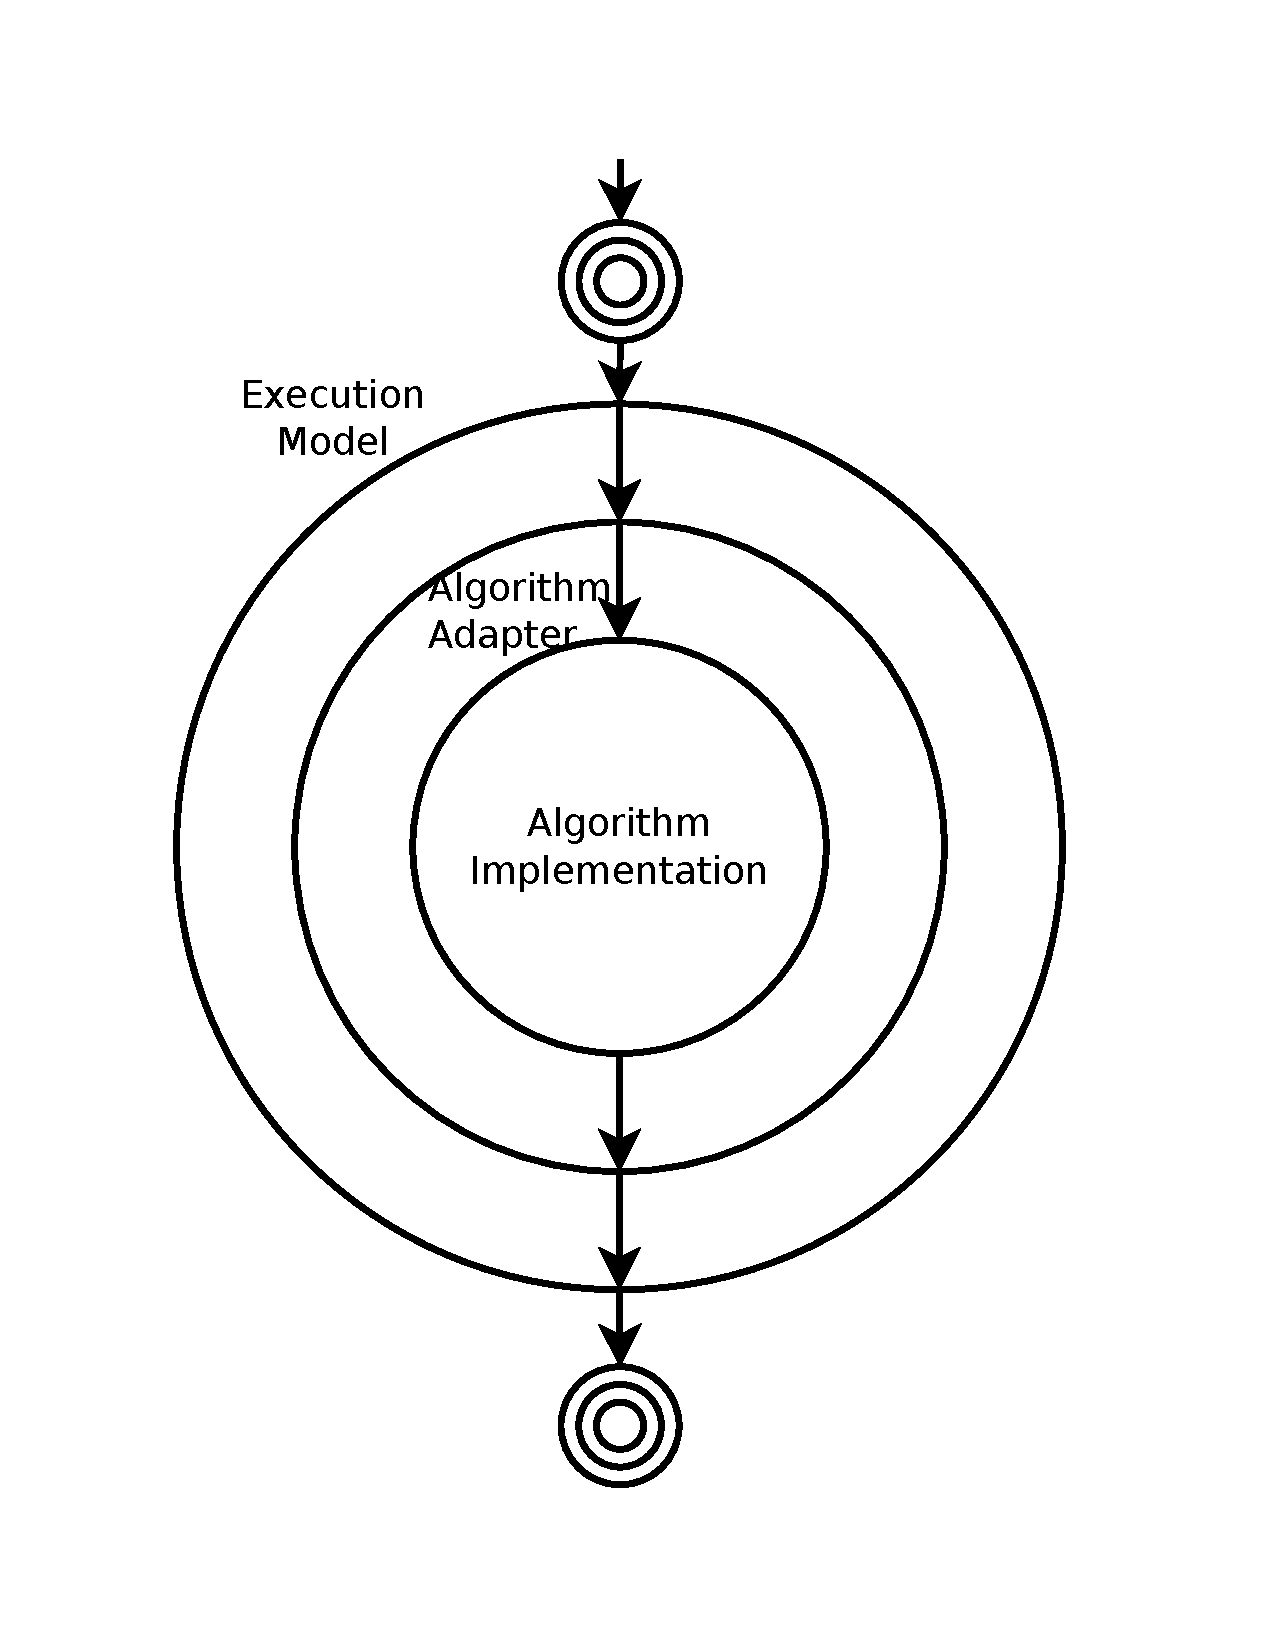
\includegraphics[width=1.1\textwidth,trim=2cm 0cm 0cm 0cm,clip]{concentric.pdf}      
    \end{column}
  \end{columns}

\end{frame}
